%!TEX TS-program = pdflatex                                          %
%!TEX encoding = UTF8                                                %
%!TEX spellcheck = en-US                                             %
%
%%%%%%%%%%%%%%%%%%%%%%%%%%%%%%%%%%%%%%%%%%%%%%%%%%%%%%%%%%%%%%%%%%%%%%
% Handout_UI_LinkAndShare.tex
% A handout to follow during the hands-on session 2 
% 
% Author: Paula Sanz Leon
% 
% 
%%%%%%%%%%%%%%%%%%%%%%%%%%%%%%%%%%%%%%%%%%%%%%%%%%%%%%%%%%%%%%%%%%%%%%
% based on the tufte-latex template                                  %

\documentclass{tufte-handout}

%\geometry{showframe}% for debugging purposes -- displays the margins

\usepackage{amsmath}

% Set up the images/graphics \underline{\textbf{Analysis}}
\usepackage[pdftex]{graphicx}
\setkeys{Gin}{width=\linewidth,totalheight=\textheight,keepaspectratio}
\graphicspath{{figures/} {../../framework_tvb/tvb/interfaces/web/static/style/img/} {../../framework_tvb/tvb/interfaces/web/static/style/img/nav/}{../../framework_tvb/tvb/interfaces/web/static/style/nodes/}}

\title{The Virtual Brain: Hands on Session \#2}
\date{7th June 2014} 

% The following package makes prettier tables.  
\usepackage{booktabs}


% The units package provides nice, non-stacked fractions and better spacing
% for units.
\usepackage{units}
\usepackage[svgnames]{xcolor}

% The fancyvrb package lets us customize the formatting of verbatim
% environments.  We use a slightly smaller font.
\usepackage{fancyvrb}
\fvset{fontsize=\normalsize}

% Small sections of multiple columns
\usepackage{multicol}

% For adjustwidth environment
\usepackage[strict]{changepage}

% For formal definitions
\usepackage{framed}

% And some maths
\usepackage{amsmath}  % extended mathematics

% Resume a list
\usepackage{enumitem}

% Background image

\usepackage{wallpaper}

% Provides paragraphs of dummy text
\usepackage{lipsum}

% These commands are used to pretty-print LaTeX commands
\newcommand{\doccmd}[1]{\texttt{\textbackslash#1}}% command name -- adds backslash automatically
\newcommand{\docopt}[1]{\ensuremath{\langle}\textrm{\textit{#1}}\ensuremath{\rangle}}% optional command argument
\newcommand{\docarg}[1]{\textrm{\textit{#1}}}% (required) command argument
\newenvironment{docspec}{\begin{quote}\noindent}{\end{quote}}% command specification environment
\newcommand{\docenv}[1]{\textsf{#1}}% environment name
\newcommand{\docpkg}[1]{\texttt{#1}}% package name
\newcommand{\doccls}[1]{\texttt{#1}}% document class name
\newcommand{\docclsopt}[1]{\texttt{#1}}% document class option name

\newcommand\blfootnote[1]{\begingroup
         \renewcommand\thefootnote{}\footnote{\phantom{\thefootnote} #1}%
         \addtocounter{footnote}{-1}%
         \endgroup
          }

% Colours: environment derived from framed.sty: see leftbar environment definition
\definecolor{formalshade}{rgb}{0.95,0.95,1}
\definecolor{simulationshade}{rgb}{0.92, 1.0, 0.95}

% Title rule
\newcommand{\HRule}{\rule{\linewidth}{0.5mm}}

% Framed  coloured boxes

%% Blue box: for steps regarding analysis and such
\newenvironment{formal}{%
  \def\FrameCommand{%
    \hspace{1pt}%
    {\color{DarkBlue}\vrule width 2pt}%
    {\color{formalshade}\vrule width 4pt}%
    \colorbox{formalshade}%
  }%
  \MakeFramed{\advance\hsize-\width\FrameRestore}%
  \noindent\hspace{-4.55pt}% disable indenting first paragraph
  \begin{adjustwidth}{}{7pt}%
  \vspace{2pt}\vspace{2pt}%
}
{%
  \vspace{2pt}\end{adjustwidth}\endMakeFramed%
}

%% Green box: for steps regarding simulatio **only**
\newenvironment{simulation}{%
  \def\FrameCommand{%
    \hspace{1pt}%
    {\color{ForestGreen}\vrule width 2pt}%
    {\color{simulationshade}\vrule width 4pt}%
    \colorbox{simulationshade}%
  }%
  \MakeFramed{\advance\hsize-\width\FrameRestore}%
  \noindent\hspace{-4.55pt}% disable indenting first paragraph
  \begin{adjustwidth}{}{7pt}%
  \vspace{2pt}\vspace{2pt}%
}
{%
  \vspace{2pt}\end{adjustwidth}\endMakeFramed%
}

%% Orange box: for verbose descriptions
\newenvironment{blah}{%
  \def\FrameCommand{%
    \hspace{1pt}%
    {\color{DarkOrange}\vrule width 2pt}%
    {\color{PeachPuff}\vrule width 4pt}%
    \colorbox{PeachPuff}%
  }%
  \MakeFramed{\advance\hsize-\width\FrameRestore}%
  \noindent\hspace{-4.55pt}% disable indenting first paragraph
  \begin{adjustwidth}{}{7pt}%
  \vspace{2pt}\vspace{2pt}%
}
{%
  \vspace{2pt}\end{adjustwidth}\endMakeFramed%
}

\begin{document}
\thispagestyle{plain}
\LLCornerWallPaper{1.5}{background.png}
\begin{titlepage}
\begin{center}
% Upper part of the page. The '~' is needed because \\
% only works if a paragraph has started.

\includegraphics[width=1.5\textwidth]{./tvb_logo_transparent_square.png}~\\[0.5cm]

% Title
\begin{fullwidth}
\HRule \\[0.2cm]
\begin{center}
{ \huge \bfseries Hands-on Session \#5 \\ [0.2cm] Modelling Epilepsy \\[0.1cm] }
{ \large \bfseries November 14, 2014 \\[0.2cm]}
\end{center}
\HRule \\[0.2cm]
\end{fullwidth}

\end{center}
\end{titlepage}

\newpage
\ClearWallPaper

\section{Objectives}\label{sec:objectives}

\newthought{This short tutorial} provides the basic steps you need to know in order to import data into TVB; share data with other users and/or link data to other TVB projects.
After this session you should be able to export a project and share it with your neighbour. 

\section{Project :Session\_II\_ShareAndLink\_a}\label{sec:project_data}
% let's start a new thought -- a new section

\subsection{Multiple Users And One Virtual Brain}\label{sec:multiusers}
In this exercise we will assume that multiple users are working with the same TVB installation. \sidenote{Working in pairs might be a good idea.} There are two simulations in one of this projects as decribed in Table \ref{tab:normaltab}.

\begin{margintable}
  \centering
  \fontfamily{ppl}\selectfont
  \begin{tabular}{l}
    \toprule
    Name \\
    \midrule
    \multicolumn{1}{l}{LinkAndShare}\\
    \textit{SimulationConnectivity74} \\
    \textit{SimulationConnectivity96} \\
    \bottomrule
  \end{tabular}
  \caption{Simulations in this project.}
  \label{tab:normaltab}
\end{margintable}


\begin{marginfigure}
  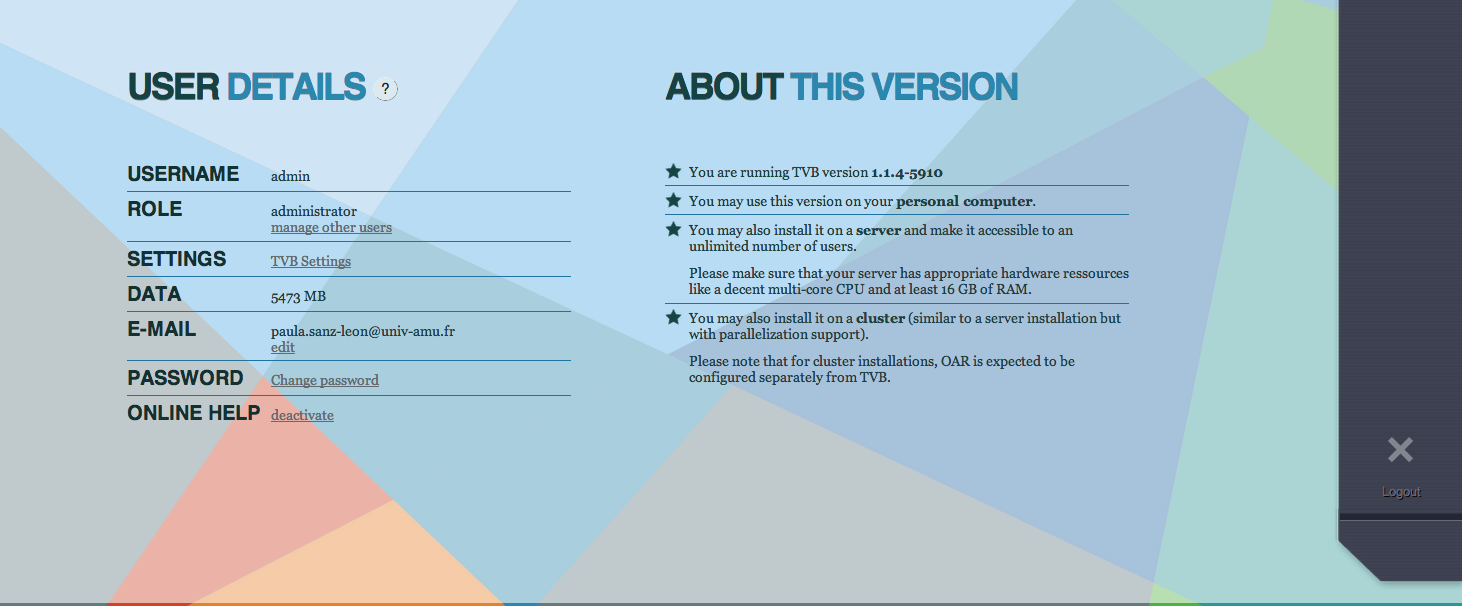
\includegraphics[width=\linewidth]{Handout_UI_LinkAndShare_ChangeAdminEmail}%
  \caption{Change \underline{Admin} email.}%
  \label{fig:change_email}%
\end{marginfigure}

\begin{marginfigure}
  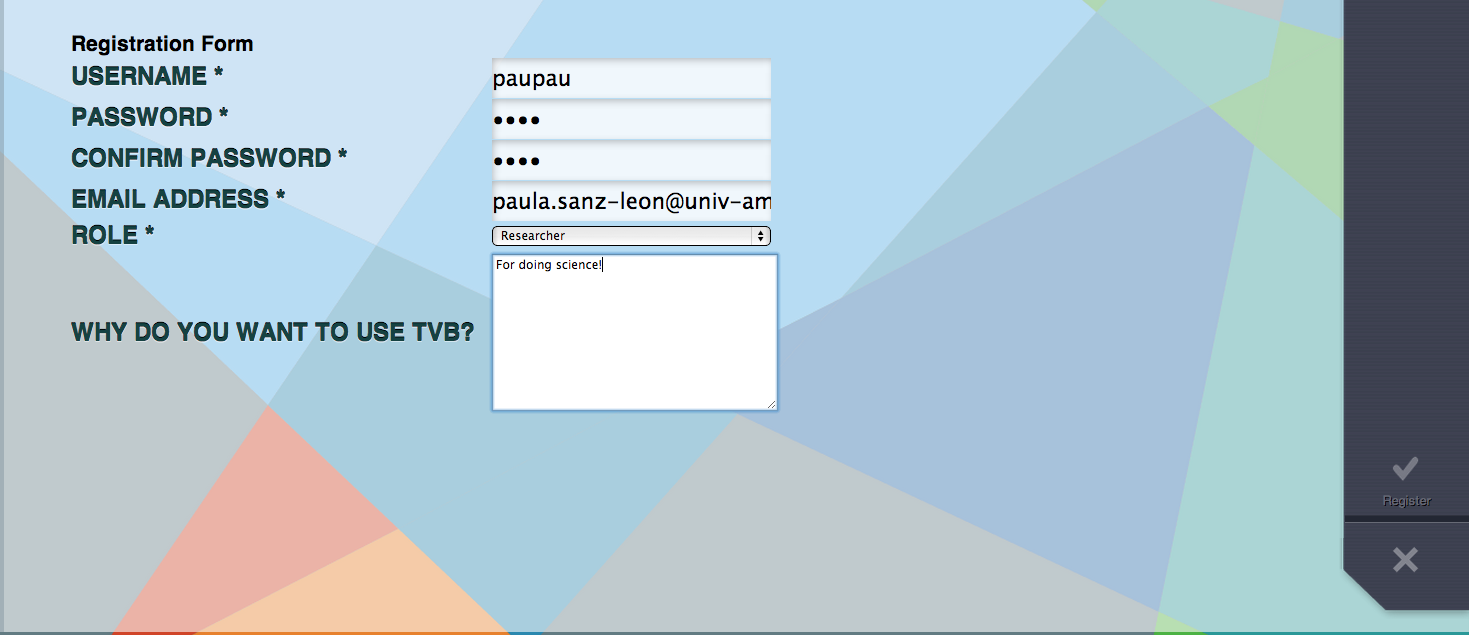
\includegraphics[width=\linewidth]{Handout_UI_LinkAndShare_AddNewUser}%
  \caption{Create a new user.}%
  \label{fig:new_user}%
\end{marginfigure}

\begin{marginfigure}
  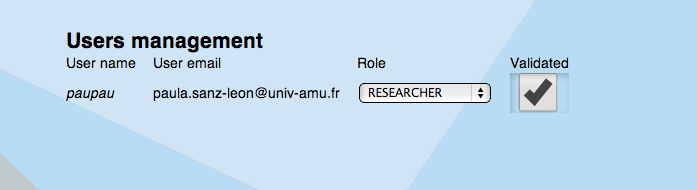
\includegraphics[width=\linewidth]{Handout_UI_LinkAndShare_ValidateNewUser}%
  \caption{Validate user.}%
  \label{fig:validate_user}%
\end{marginfigure}

\begin{formal}
\begin{enumerate}
\item By default your are the \underline{Admin} user. 
\item Change the admin email (Fig. \ref{fig:change_email}).
\item Create a user for your neighbour by registering a new user. (Fig. \ref{fig:new_user}). 
\item You'll receive a notification email.
\item Make sure the new user has been validated. (Fig. \ref{fig:validate_user}).
\item Login with the \underline{Admin} account. 
\end{enumerate}
\end{formal}

\subsection{Importing A Connectivity}\label{sec:import_connectivity}

\begin{formal}
\begin{enumerate}
\item Create a project (e.g. \textit{Session\_II\_LinkAndShare\_a}). 
\item Create a second project (e.g. \textit{Session\_II\_LinkAndShare\_b}). 
\item Assuming that you are working in the first project, upload a \underline{Connectivity} in a zip file. This was already done but you can repeat these steps. 
\item Go to \textsc{Projects}$\rightarrow$ \textsc{Data structure}. Click on \underline{Upload Data}. An overlay with the current supported formats will appear. See Fig. \ref{fig:uploaders}. 
\item Select \underline{Connectivity ZIP}. 
\item Select the file \textit{connectivity\_regions\_96.zip} found at \textit{TVB\_Distribution/tvb\_data/}.
\end{enumerate}
\end{formal} 

\begin{figure}[h]
  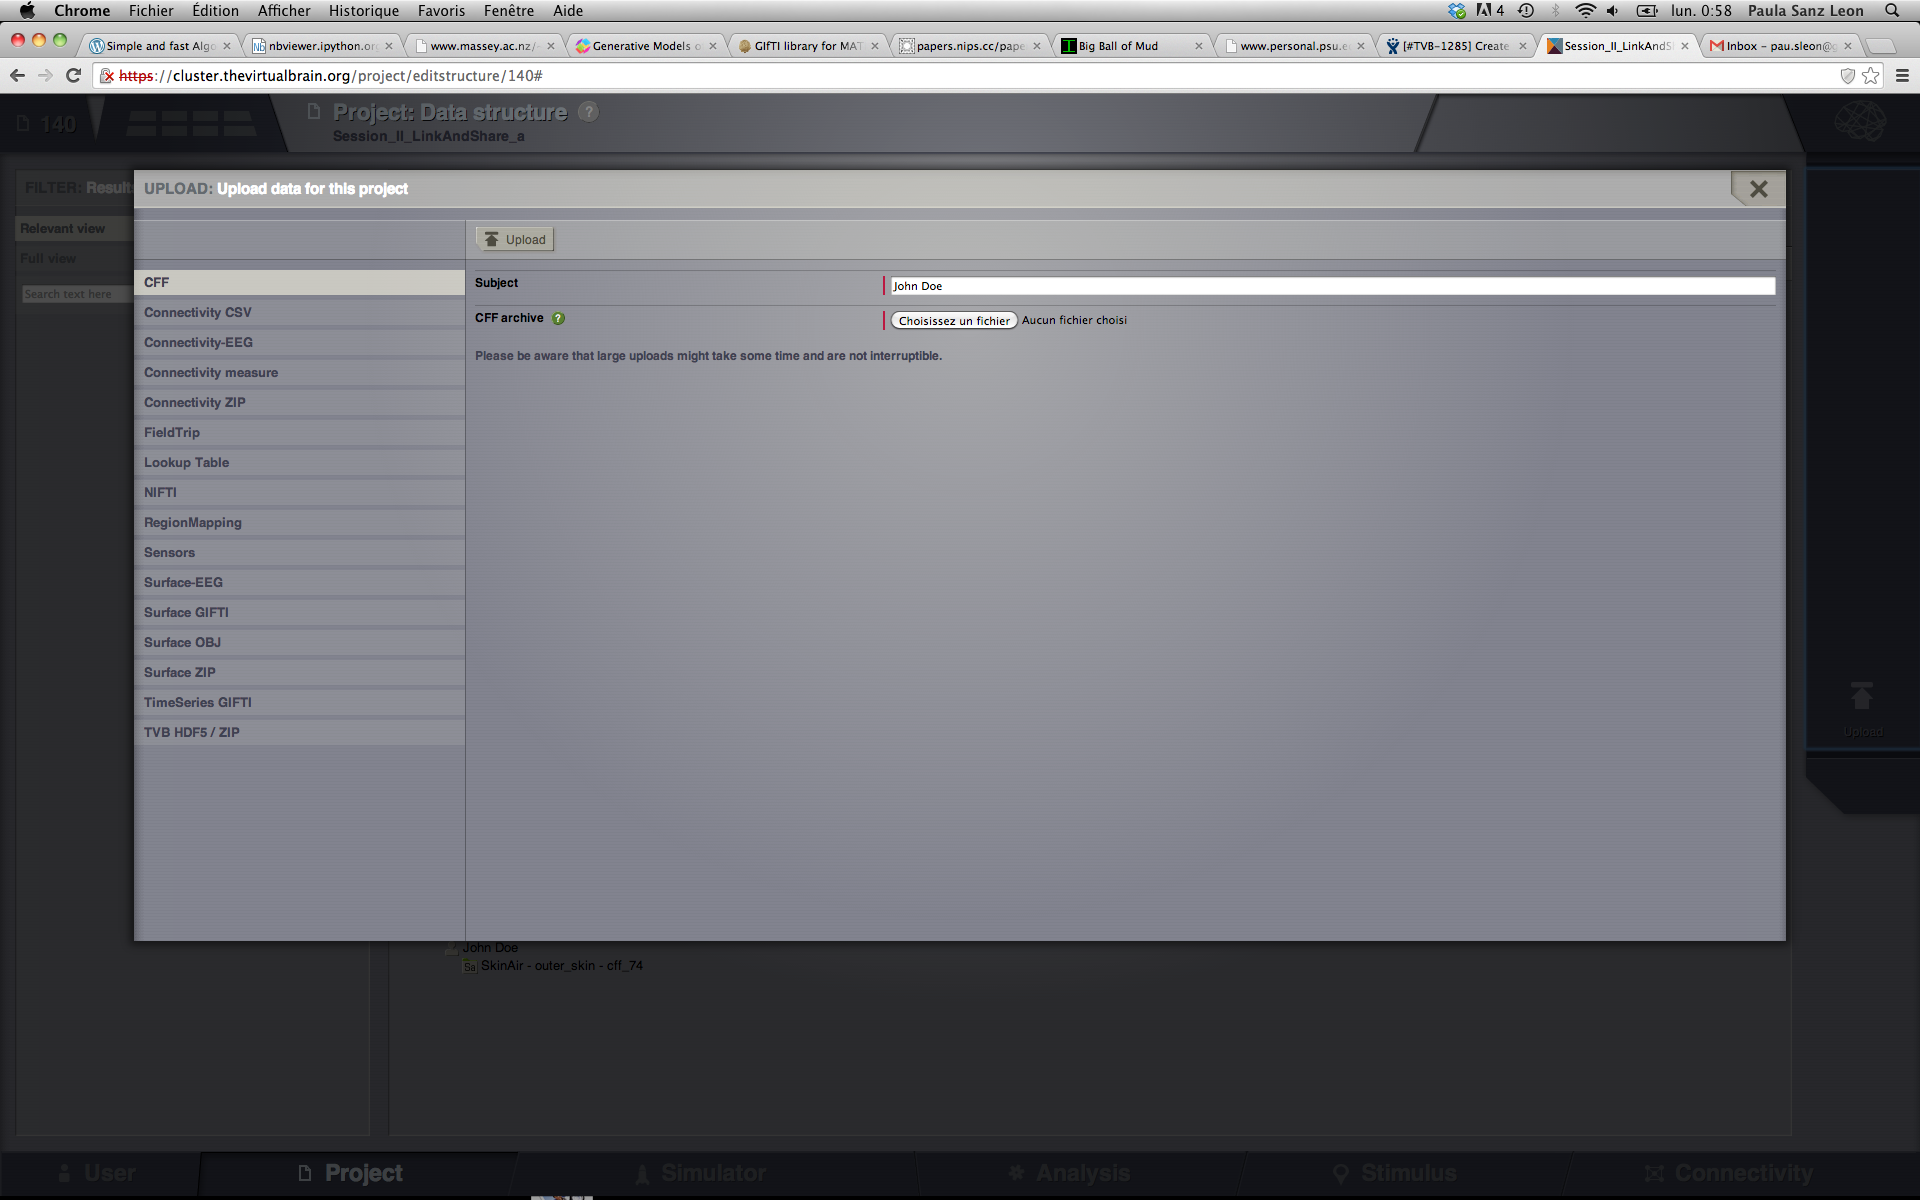
\includegraphics[width=\linewidth]{Handout_UI_LinkAndShare_Uploaders}%
  \caption{Supported data formats.}%
  \label{fig:uploaders}%
\end{figure}


\begin{formal}
\begin{enumerate}[resume]
\setcounter{enumi}{6}
\item Add a personalized tag to this newly created datatype (e.g. \textit{conn\_96}).  See Fig. \ref{fig:tag}. 
\item Save the changes.
\end{enumerate}
\end{formal}

\begin{figure}[h]
  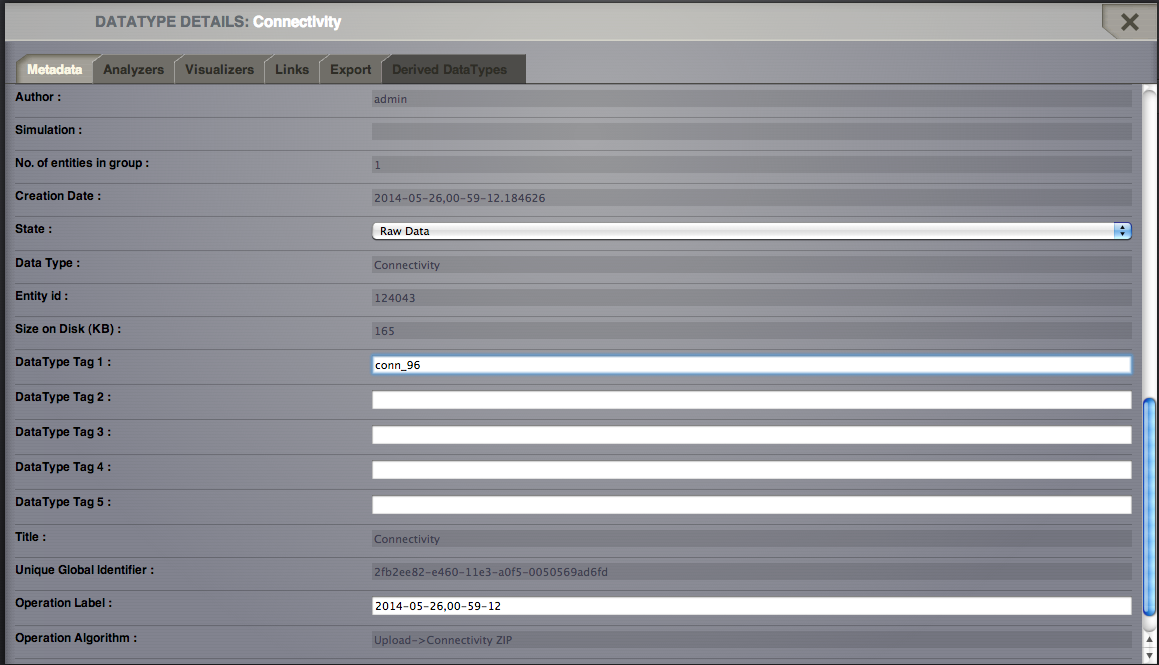
\includegraphics[width=\linewidth]{Handout_UI_LinkAndShare_TagDatatype}%
  \caption{Add a personalized tag.}%
  \label{fig:tag}%
\end{figure}


\subsection{Link And Share}\label{sec:link_and_share}
\begin{formal}
\begin{enumerate}[resume]
\setcounter{enumi}{8}
\item Select the connectivity you want to share.
\item In the \underline{metadata overlay}. Go to the tab \underline{Links}. You'll see a list with all your projects. See Fig. \ref{fig:linkstab}.
\item Link this datatype (connectivity) with the project you'll share (e.g. \textit{Session\_II\_ShareAndLink\_b}).
\item Link the two time-series from simulations \textit{SimulationConnectivity74} and \textit{SimulationConnectivity96}.
\end{enumerate}
\end{formal} 

\begin{figure}[h]
  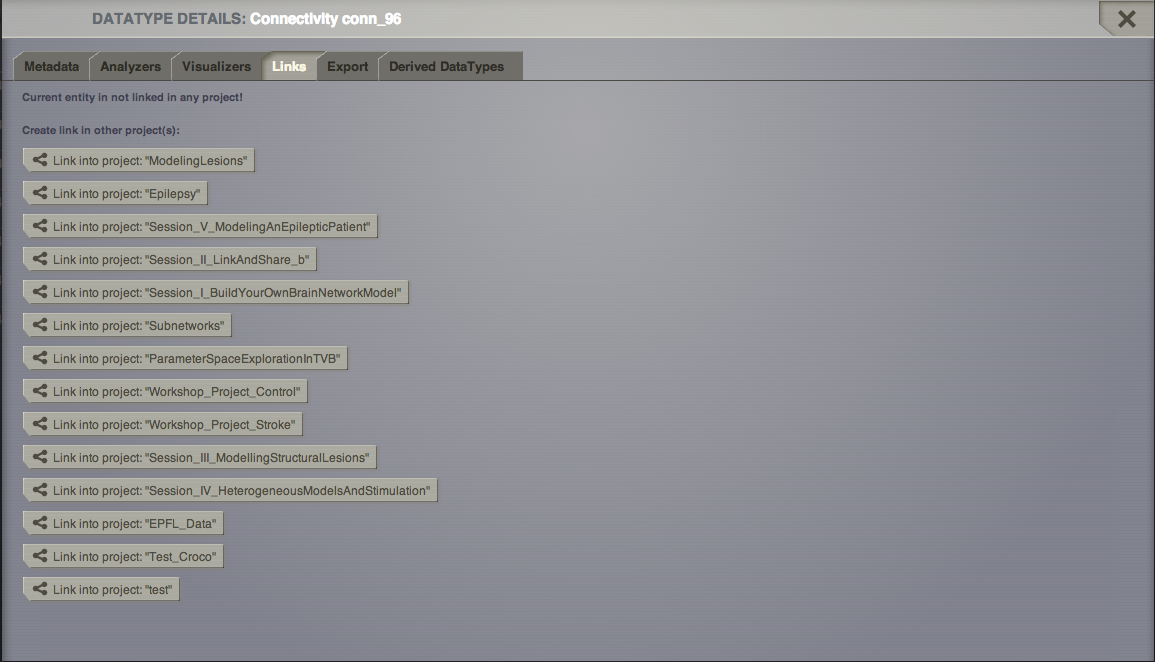
\includegraphics[width=\linewidth]{Handout_UI_LinkAndShare_LinksTab}%
  \caption{Links tab.}%
  \label{fig:linkstab}%
\end{figure}

\begin{figure}[h]
  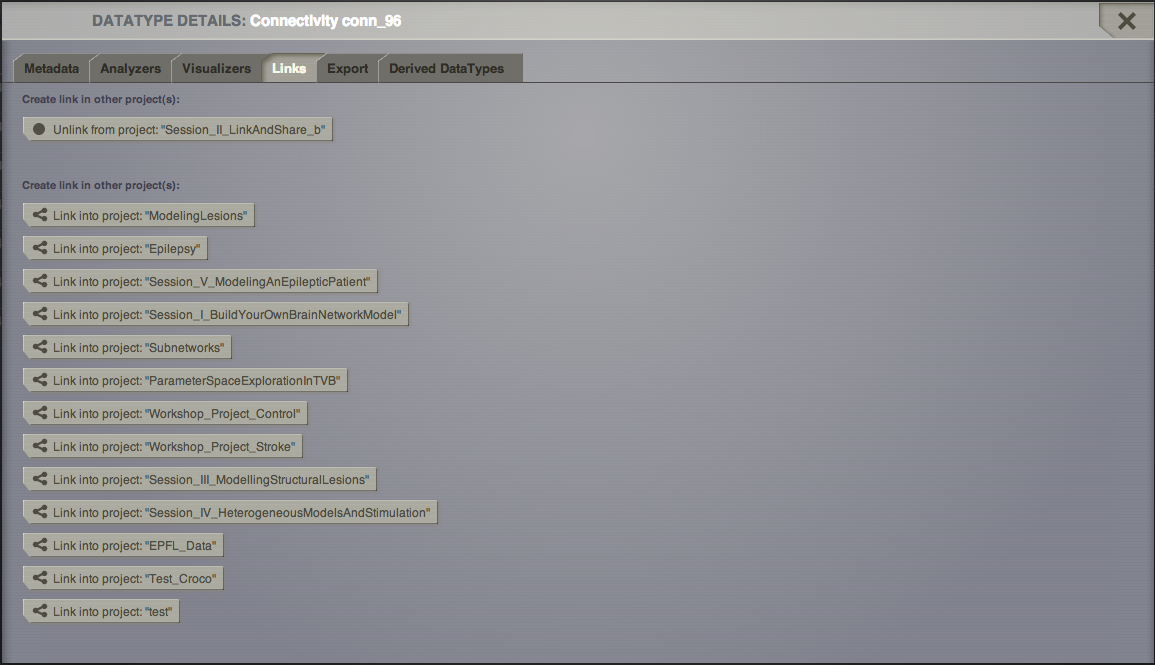
\includegraphics[width=\linewidth]{Handout_UI_LinkAndShare_LinkedProject}%
  \caption{Link a datatype to another project.}%
  \label{fig:linkproject}%
\end{figure}

\begin{formal}
  \begin{enumerate}[resume]
    \setcounter{enumi}{10}
    \item Go to \textsc{Project} $\rightarrow$ \textsc{List of all projects}
    \item Switch to \textit{Session\_II\_ShareAndLink\_b}.
    \item Then from \textsc{Project} $\rightarrow$ \textsc{Basic properties} 
share this project with your neigbour's user account. 
    \item Logout from your account and let your neighbour login to his/her account. 
  \end{enumerate}
\end{formal} 

\begin{blah}
You should be able to see the connectivity matrix (and other datatypes) you linked
from project \textit{Session\_II\_ShareAndLink\_a}.
\end{blah}

\subsection{Export and Read}\label{sec:link_and_share}

\begin{formal}
  \begin{enumerate}
    \item Go to \textsc{Project} $\rightarrow$ \textsc{Data structure}
    \item Click on 
\includegraphics[width=0.01\textwidth]{nodeTimeSeriesRegion.png} from \textit{TimeSeriesRegion - conn\_74}. 
    \item From the overlay, \underline{Export} tab, download the data in TVB format (h5).
    \item Rename the file if you want (e.g. \textit{LinkAndShare\_TimeSeriesRegion}).
    \item From an ipython shell you can follow the commmands presented below. 
  \end{enumerate}
\end{formal} 

\begin{blah}
\begin{verbatim}
In [1]: import h5py
In [2]: import matplotlib.pyplot as plt

In [3]: f = h5py.File('LinkAndShare_TimeSeriesRegion.h5')

In [4]: f.keys()
Out[4]: [u'data', u'time']

In [5]: f.attrs.keys()
Out[5]: 
[u'TVB_User_tag_1',
 u'TVB_Title',
 u'TVB_Length_2d',
 u'TVB_Gid',
 u'TVB_Length_3d',
 u'TVB_Sample_period_unit',
 u'TVB_Labels_ordering',
 u'TVB_Length_1d',
 u'TVB_User_tag_4',
 u'TVB_User_tag_5',
 u'TVB_Subject',
 u'TVB_Length_4d',
 u'TVB_Data_version',
 u'TVB_User_tag_3',
 u'TVB_Is_nan',
 u'TVB_Type',
 u'TVB_Invalid',
 u'TVB_Connectivity',
 u'TVB_Create_date',
 u'TVB_User_tag_2',
 u'TVB_Labels_dimensions',
 u'TVB_Sample_rate',
 u'TVB_State',
 u'TVB_Start_time',
 u'TVB_Sample_period',
 u'TVB_Nr_dimensions',
 u'TVB_Visible',
 u'TVB_Module']


In[6]: plt.plot(f['time'], f['data'][:, 0, :, 0])
...

In [7]: plt.xlabel('time [ms]')
Out[7]: <matplotlib.text.Text at 0x118e95310>

In [8]: plt.ylabel('amplitude [au]')
Out[8]: <matplotlib.text.Text at 0x118e9a190>

In [9]: plt.title(f.attrs['TVB_Title'])
Out[9]: <matplotlib.text.Text at 0x118eb0ad0>
\end{verbatim}
\end{blah}


\begin{figure}[h]
  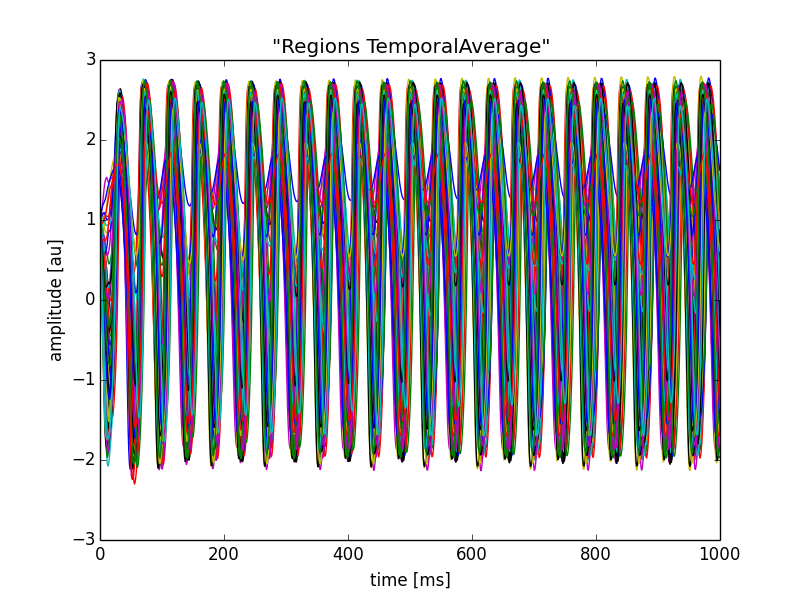
\includegraphics[width=\linewidth]{Handout_UI_LinkAndShare_IpythonTimeSeriesRegion.png}%
  \caption{Plotting time-series with matplotlib.}%
  \label{fig:ipython}%
\end{figure}

In matlab \sidenote{hdf5read will be removed in a future version. Use h5read instead.}:

\begin{verbatim}
>> hinfo = hdf5info('LinkAndShare_TimeSeriesRegion.h5');
>> hinfo.GroupHierarchy.Datasets.Name

ans =

/data


ans =

/time


>> hinfo.GroupHierarchy.Attributes.Name

...


>> data = hdf5read(hinfo.GroupHierarchy.Datasets(1));
>> time = hdf5read(hinfo.GroupHierarchy.Datasets(2));
>> plot(time, squeeze(data))
>> xlabel('time [ms]')	
>> ylabel('amplitude [au]')

\end{verbatim}

\begin{figure}[h]
  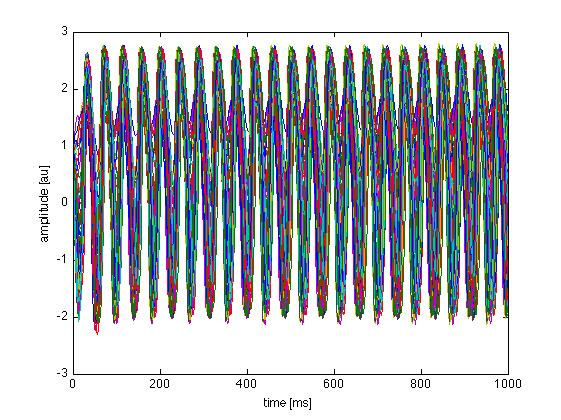
\includegraphics[width=\linewidth]{Handout_UI_LinkAndShare_MatlabTimeSeriesRegion.png}%
  \caption{Plotting time-series with matlab.}%
  \label{fig:matlab}%
\end{figure}

In R \sidenote{You need the rhdf5 package}:

\begin{verbatim}
> data <- h5read("/Users/paupau/GithubProjects/tvb-handbook/
tvbworkshop/LinkAndShare_TimeSeriesRegion.h5", "data")

> time <- h5read("/Users/paupau/GithubProjects/tvb-handbook/
tvbworkshop/LinkAndShare_TimeSeriesRegion.h5", "time")

> data = drop(mydata)

> plot(mytime, data[,1], type="l")
\end{verbatim}

\begin{figure}[h]
  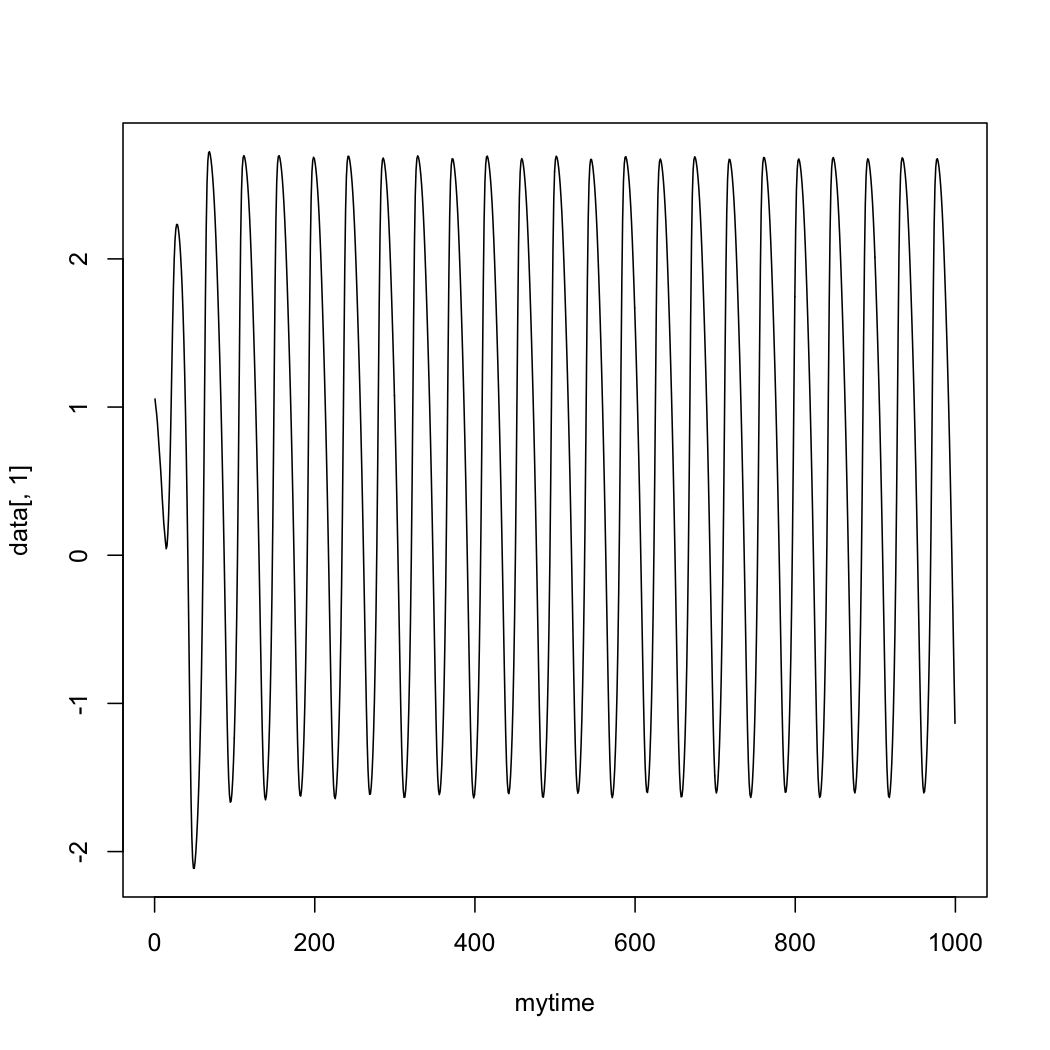
\includegraphics[width=\linewidth]{Handout_UI_LinkAndShare_RTimeSeriesRegion.png}%
  \caption{Plotting time-series with R.}%
  \label{fig:r}%
\end{figure}



\section{More Documentation}\label{sec:more-doc}

For more details on technical aspects of The Virtual Brain, please see the following articles
\citep{Sanz-Leon_2013, Woodman_2014}

\section{Support}\label{sec:support}

The official TVB webiste is \url{www.thevirtualbrain.org}.  
All the documentation and tutorials are hosted on \url{the-virtual-brain.github.io}.
You'll find our public \smallcaps{git} repository at \url{https://github.com/the-virtual-brain}. 
For questions and bug reports we have a users group \url{https://groups.google.com/forum/#!forum/tvb-users}

\bibliography{tvb_references}
\bibliographystyle{plainnat}

\end{document}


































































